\graphicspath{{./images/}}

\chapter{Verteilungssicht}
\label{deploy}

\section{Aufbau}
Die Software wird auf der neu, aktuell im Aufbau befindenden, Containerplattform OpenShift installiert. Das genaue Deployment des Clusters ist Aufgrund von Abklärungen betreffend PCI DSS Compliance noch nicht abschliessend definiert. Konzeptionell ändert sich jedoch nicht viel da für die Applikation der Aufbau der Umgebung transparent ist.
OpenShift verwendet diverse Konzepte welche kurz erläutert werden soll, und sich im Diagramm im Kapitel \ref{deploy-dia} wieder finden. Im Kapitel \ref{config} finden sich sämltich Informationen im Bezug auf die Konfiguration.

\subsection{Container und Pods}

Neben den normalen Docker Container kenn OpenShift das Konzept von Pods. Pods\footnote{https://kubernetes.io/docs/user-guide/pods/} sind logisch gruppierte Einheiten von Docker Containern, des gleichen Types, welche gemeinsame Resourcen, IP Addressen, Speicher usw.,  aufweisen. Pods sind wie Container sterblich und werden von OpenShift beim hoch- oder runterskaliere respektive bei Fehlern einfach gelöscht und gegebenenfalls als neue Instanz gestartet. Detailierte Informationen zu Containern finden sich im Kapitel \ref{container}.

\subsection{Services}

Services\footnote{https://kubernetes.io/docs/user-guide/services/} sind eine weitere Abstraktion von OpenShift welche Pods gruppiert. Wenn verschiedene Pods miteinander kommunizieren wollen, braucht es eine Möglichkeite den Netzwerkverkehr zu organisieren. Services sind die Schnittstelle zwischen einzelnen Pods welche intern wie ein Loadbalancer funktionieren, welche eine Anfrage an einen Pod weiterleiten. Durch diesen Mechanismus wird es möglich dynamisch Pods hinzu zufügen oder zu entfernen.


\section{Diagramm}
\label{deploy-dia}
\begin{center}
	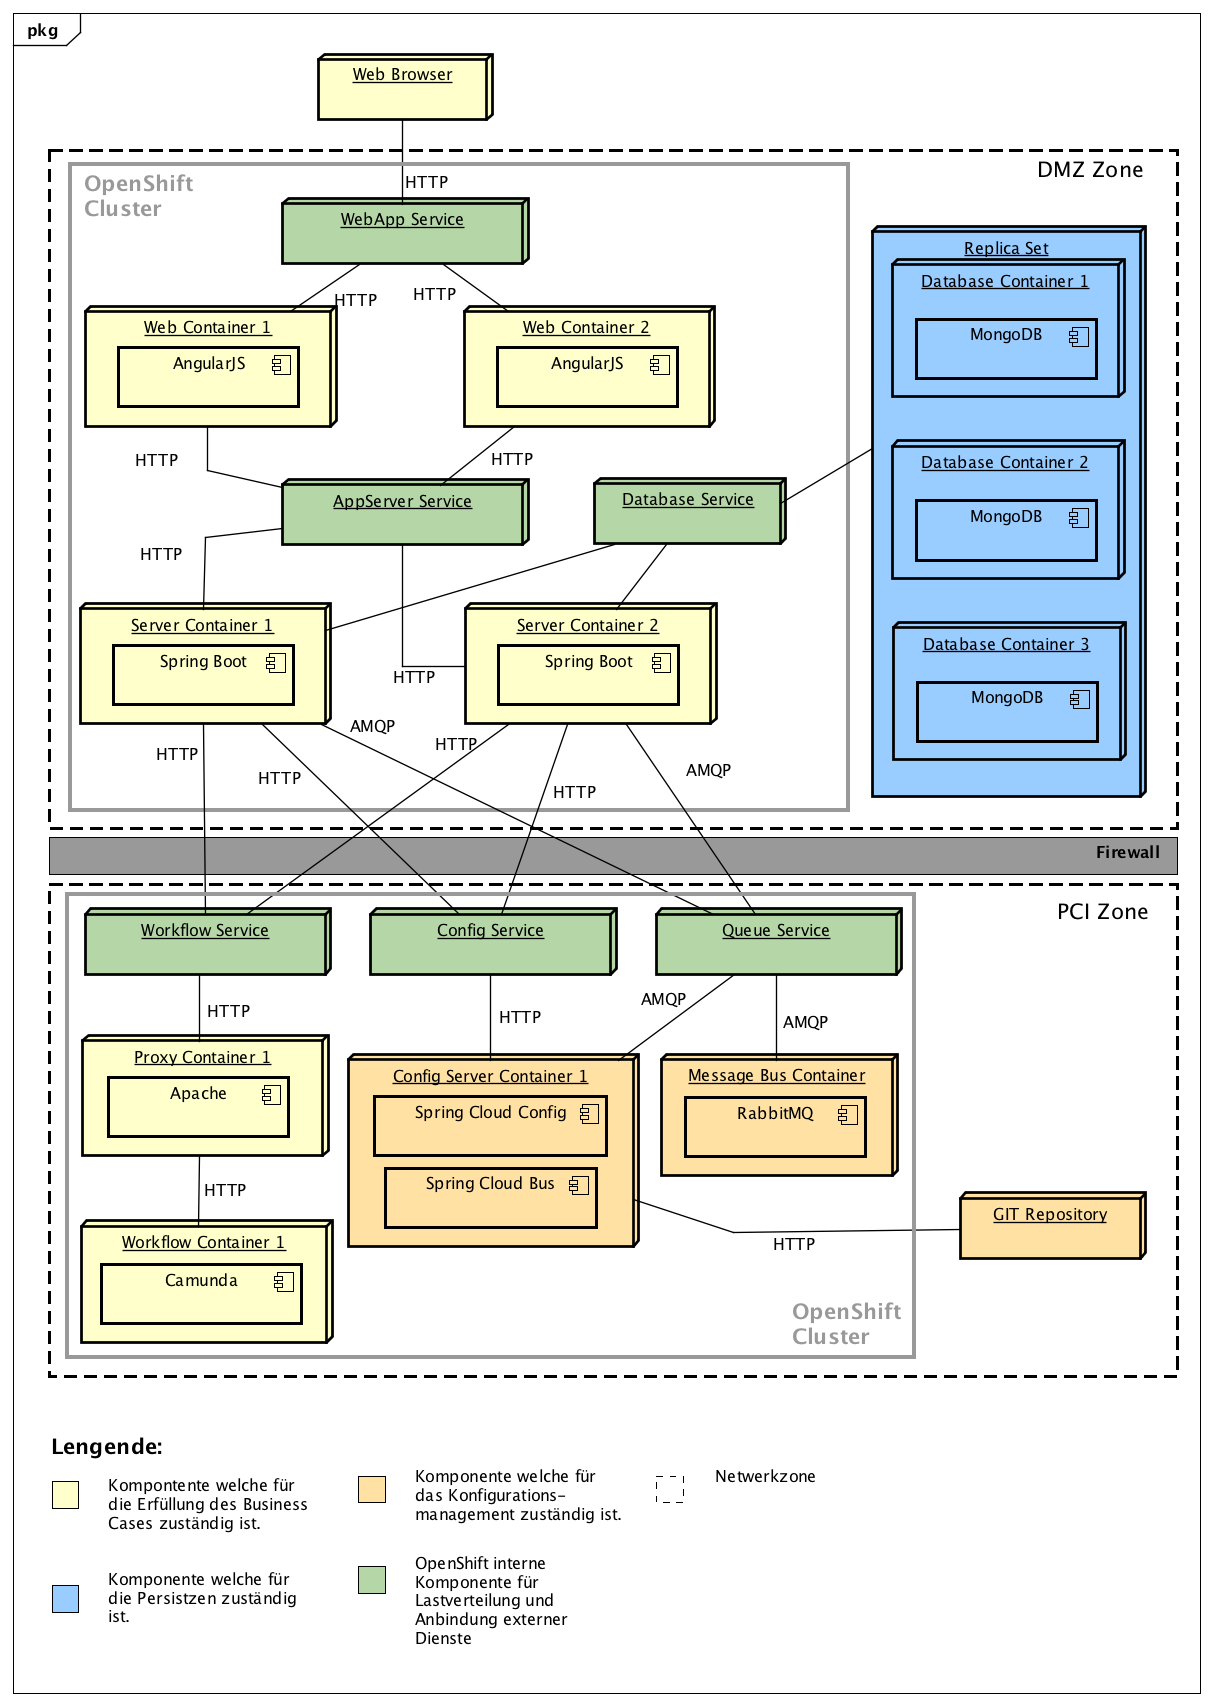
\includegraphics[scale=0.45]{OpenShiftDeployment.png}
\end{center}

\section{Aufbau}

In der Verteilungssicht gibt es folgende Komponenten:\newline
\begin{itemize}
	\item Geld sind die Teile welche den Use Case der Applikation abbilden und es dem Benutzer ermöglichen sich für Twint anzumelden. Dazu gehören der WebServer mit dem statischen Inhalt für die WebPage, der Serverteil sowie die Workflow Enginge.
	\item Orange sind Komponenten welche für das Konfigurationsmanagement der Applikation verantwortlich sind. Hierzu gehört eine Spring Boot Anwendung, ein Message Bus für die benachrichtigung der Server sowie ein GIT-Repository welches die Konfigurationen, gespeichert in Property files, beinhaltet.
	\item Grün sind OpenShift Services welche die Schnittstellen zwischen den einzelnen Teilen der gesamt Applikation verbinden.
	\item Blau sind Teile welche für die Datenspeicherung verwendet werden. Es handelt sich dabei um ein Replica Set von MongoDB mehr Informationen zur Persistzen finden sich im Kapitel \ref{persistenz}.
\end{itemize}

Aus Compliance Gründen befindet sich die Workflow Engine sowieo die Config Server in einer separaten, durch eine Firewall getrennten, Zone innerhalb des Clusters. Da die Workflow Engines auf Dienste welche mit Kreditkartendaten zugreifen muss, fällt die Komponente automatisch unter die gleichen Regeln. 

